%% =============================================================================
%% ===========      MATERIAIS E METODOS            =============================
%% =============================================================================
\chapter{Materiais e Métodos}
\label{chap:mat_met}

Nesta seção serão apresentados os materiais e métodos que serão utilizados para o desenvolvimento do projeto.

%================================================================================
\section{Visão geral do sistema proposto}
\label{sec:visaoGeralSist}

O sistema proposto consiste em um RMA composto por um Raspberry Pi, um Arduino, sensores e atuadores fixados em um chassi redondo. O Raspberry Pi tem a finalidade de obter e processar a imagem a partir de um método de visão computacional da biblioteca OPENCV, adquirindo a informação necessária e transmitindo-a para o Arduino, onde o sistema de controle estará embarcado e atuará nos motores de acordo com a movimentação necessária. Um conjunto de sensores ultrassônicos será responsável pela percepção de algum objeto que poderá impedir a trajetória inicialmente definida.

Na Figura~\ref{fig:sistema-proposto} pode-se observar um esboço dos cargos de cada placa no sistema.

\begin{figure}[!hbtp]
  \centering
   \caption{Sistema Proposto}
    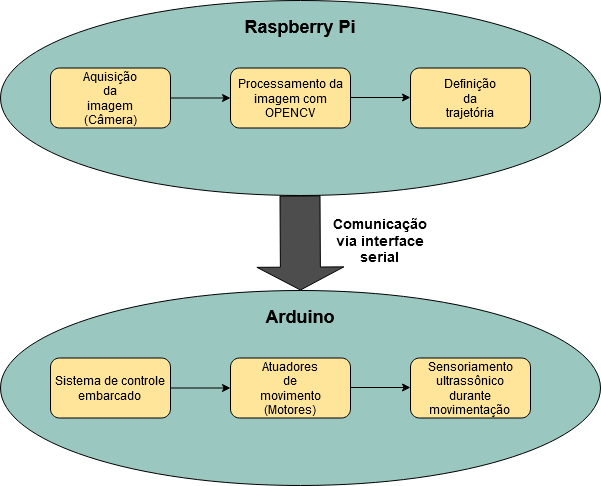
\includegraphics[width = 0.8\textwidth]{Caps/Figs/mat-met/Sistema-proposto.png}
   \label{fig:sistema-proposto}
    \fonte{Autor}
\end{figure}

\nomenclature{RMA}{Robô Móvel Autônomo}

%================================================================================
\section{Arduino}
\label{sec:Arduino}

O Arduino consiste em uma plataforma de prototipagem eletrônica com placa única e hardware livre. É projetado com um microcontrolador RISC Atmel AVR de chip único, com suporte embutido de entradas e saídas e linguagem de programação padrão que é essencialmente C/C++. Este pode receber sinais elétricos, analisá-los e tomar decisões para a ação dos atuadores a ele conectados, como relés, motores, servomotores, entre outros.

Neste projeto será utilizado um Arduino UNO, mostrado na Figura~\ref{fig:arduino-uno}, que possui 14 pinos de entrada/saída digital (dos quais 6 podem ser usados como saídas PWM), 6 entradas analógicas, um cristal oscilador de 16MHz, uma porta de conexão universal (USB - \textit{Universal Serial Bus}), uma entrada de alimentação e um botão de reset.

\begin{figure}[!hbtp]
  \centering
   \caption{Arduino UNO}
    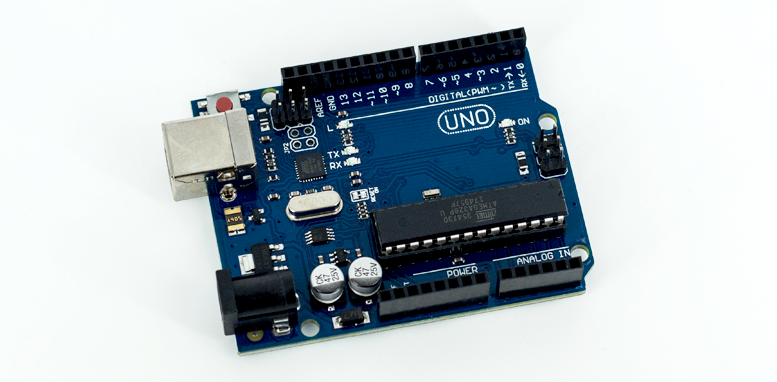
\includegraphics[width = 0.8\textwidth]{Caps/Figs/mat-met/arduino.png}
   \label{fig:arduino-uno}
    \fonte{Site\protect\footnotemark}
\end{figure}
\footnotetext{Disponível em: \url{https://uploads.filipeflop.com/2014/09/01.png}. Acesso em: 8 set. 2020.}

Para o software será utilizado o ambiente de desenvolvimento integrado (IDE - \textit{Integrated Development Environment}) disponibilizado pelo próprio Arduino para download em seu site oficial.

\nomenclature{IDE}{\textit{Integrated Development Environment}}
\nomenclature{USB}{\textit{Universal Serial Bus}}

%================================================================================
\section{Raspberry Pi}
\label{sec:raspberrypi}

Raspberry Pi é um computador de placa única de tamanho reduzido que se conecta com periféricos. O dispositivo foi criado no Reino Unido pela Fundação Raspberry Pi, uma organização sem fins lucrativos, focada na promoção e no ensino de ciência da computação básica para jovens em escolas e universidades da Europa, com produtos de preço acessível. A Fundação nasceu em 2006, quando um grupo de cientistas do Laboratório de Computação da Universidade de Cambridge, no Reino Unido começou a trabalhar em um microcomputador baseado no Atmel ATmega644, que serviria de base para o Raspberry Pi.

Ele é um mini-microcomputador que, no exíguo espaço equivalente a um cartão de crédito, abriga processador, processador gráfico, \textit{slot} para cartões de memória, interface USB, uma interface condutiva digital de áudio e vídeo que permite transmitir dados não comprimidos (HDMI - \textit{High-Definition Multimedia Interface}) e  seus respectivos controladores. Além disso, ele também apresenta memória RAM, entrada de energia e barramentos de expansão.

Como visto na Figura~\ref{fig:RaspberryPi-CAM}, ele suporta diversos tipos de conectividade e possui quarenta pinos de propósito geral entrada/saída.

\begin{figure}[!hbtp]
  \centering
   \caption{Raspberry Pi}
    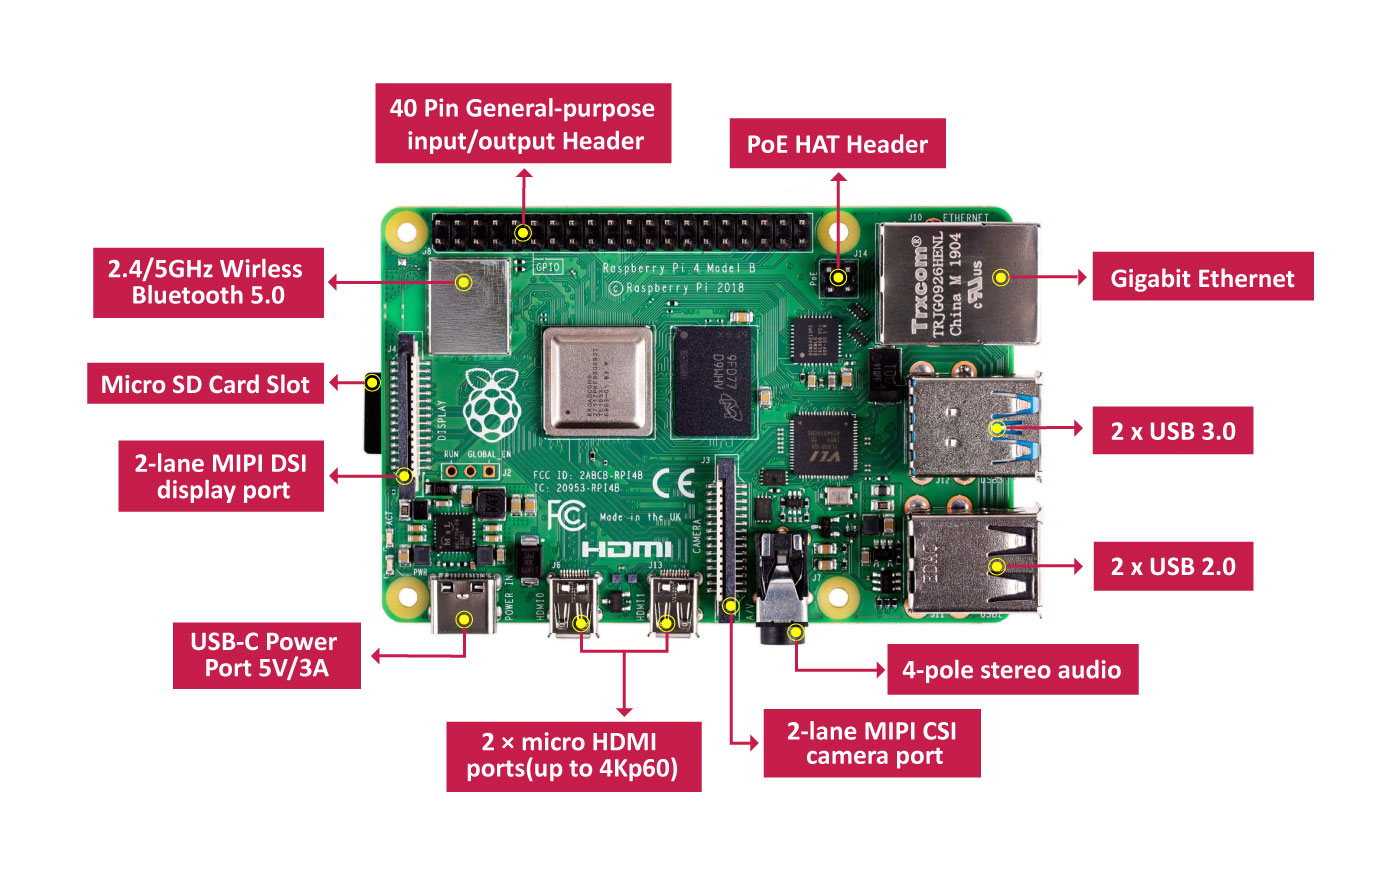
\includegraphics[width = 0.8\textwidth]{Caps/Figs/mat-met/raspberryPI.jpg}
   \label{fig:RaspberryPi-CAM}
    \fonte{Site\protect\footnotemark}
\end{figure}
\footnotetext{Disponível em: \url{https://raw.githubusercontent.com/SeeedDocument/Raspberry-Pi-4/master/img/hardware-overview-1400.jpg}. Acesso em: 8 set. 2020.}

\nomenclature{HDMI}{\textit{High-Definition Multimedia Interface}}

%================================================================================
\section{Robô Móvel}
\label{sec:robomovel}

Os robôs estão presentes no dia a dia da humanidade de diversas formas, seja ela em processos industriais, residências ou internet bot (softwares para simulação de ação humana). Ao longo dos últimos anos o interesse está em volta dos RMAs, capazes de identificar e se deslocar no ambiente que estão inseridos. Estes são classificados de acordo com o meio em que se movem, sendo ele terrestre, subaquático ou aéreo.

Quando se projeta um robô móvel deve se considerar o tipo de ambiente que ele atuará \cite{rogeralex1999}. Estes ambientes são classificados em estruturados, semi-estruturados e não-estruturados. Em um ambiente estruturado, o robô tem conhecimento prévio da quantidade e localização dos objetos. Logo, um ambiente que não é alterado, resultando em um mapa fixo de rotas possíveis do robô. Um ambiente semi-estruturado é considerado fechado e possui terreno não acidentado, mas seus limites são desconhecidos. Por fim, em um ambiente não-estruturado, o robô não possui nenhum conhecimento a respeito dos objetos ou terreno, podendo ser constantemente modificado. Exige-se então um robô com maior autonomia, capaz de se adequar ao ambiente dinâmico.

Os RMAs tem como características fundamentais as capacidades de locomoção e de operação de modo semi ou completamente autônomo. Também deve ser considerado que maiores níveis de autonomia serão alcançados somente à medida que o robô passe a integrar outros aspectos considerados de maior importância, como: capacidade de percepção (sensores que conseguem "ler" o ambiente onde ele atua), capacidade de agir (atuadores e motores capazes de produzir ações, tais como o deslocamento do robô no ambiente), robustez e inteligência (capacidade de lidar com as mais diversas situações, de modo a resolver tarefas por mais complexas que sejam) \cite{wolf2009robotica}.

%================================================================================
\section{Sensores}
\label{sec:sensores}

Um sensor pode ser definido como um dispositivo projetado para quantificar ou detectar parâmetros específicos por meio de elementos transdutores \cite{rogeralex1999}. 
Múltiplos sensores são utilizados em RMAs para o aumento de seu nível de autonomia, neste trabalho serão utilizados sensores ultrassônicos e um sensor de imagem para visão artificial.

Os sensores individualmente fornecem apenas uma "visão de mundo", parcial, incompleta e sujeita a erros, sendo papel do sistema de controle adquirir, unificar e tratar estas informações de forma robusta e inteligente \cite{wolf2009robotica}.

\subsection{Sensores Ultrassônicos}
\label{subsec:sensores-ultrassônicos}

Os sensores ultrassônicos emitem energia sonora em cones, conforme a Figura~\ref{fig:sensor-ultrassonico}, e sua diretividade depende do ângulo de abertura deste cone. É formado por um emissor e um receptor dispostos tanto juntos como separados, dependendo da configuração desejada. É o princípio de um sonar.

\begin{figure}[!hbtp]
  \centering
   \caption{Sensor Ultrassônico}
    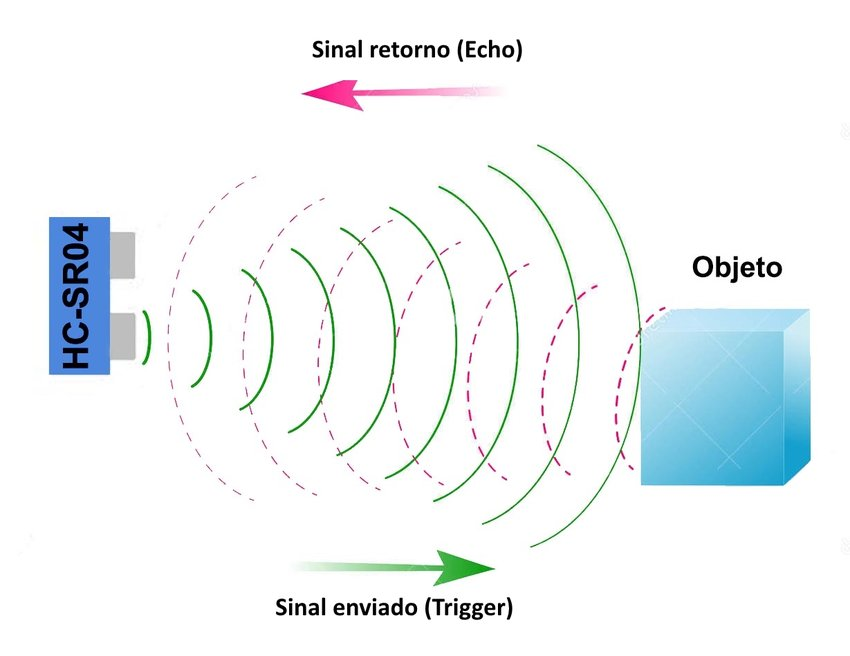
\includegraphics[width = 0.8\textwidth]{Caps/Figs/mat-met/ultrassonico.jpg}
   \label{fig:sensor-ultrassonico}
    \fonte{Site\protect\footnotemark}
\end{figure}
\footnotetext{Disponível em: \url{https://www.researchgate.net/figure/Figura-4-Funcionamento-do-sensor-ultrassonico-HC-SR04-Fonte-Site-Filipeflop-2_fig4_331135149}. Acesso em: 8 set. 2020.}

\subsection{Sensor de Imagem Utilizando Visão Artificial}
\label{subsec:sensores-imagensVisão}

A visão é o sentido mais poderoso e complexo do ser humano. É através dela que ele recebe uma grande quantidade de informações a respeito do mundo que o cerca, o que facilita interagir inteligentemente com o ambiente dinâmico. Utilizando informações visuais, o homem é capaz de estimar a posição de objetos (relativa a ele mesmo ou relativa a outros objetos), identificar formas, perceber movimentos e estimar dimensões. Tudo isso sem contato direto com os objetos \cite{rogeralex1999}.
Constantemente, há o empenho de pesquisadores para prover aos RMAs um sistema de sensoriamento capaz de desempenhar as funções da visão humana, porém ainda estão longe de obter a precisão e velocidade de processamento de informações.

Um sensor de imagem, comporta-se como a retina dos olhos, capta a luminosidade das imagens que são projetadas sobre ele continuamente e dá início ao processo de captura de uma instância ou de uma sequência de instâncias da imagem consecutivamente. Trata-se de um chip que pode contar com dezenas de milhões de transdutores fotossensíveis, cada um deles é capaz de converter a energia luminosa de um ponto da imagem em carga elétrica para ser lida ou gravada posteriormente na forma de imagem digitalizada em valores numéricos. Na Figura~\ref{fig:sensor-camRaspberry} tem-se um exemplo de câmera compatível com Raspberry Pi. 

\begin{figure}[!hbtp]
  \centering
   \caption{Câmera compatível com Raspberry Pi}
    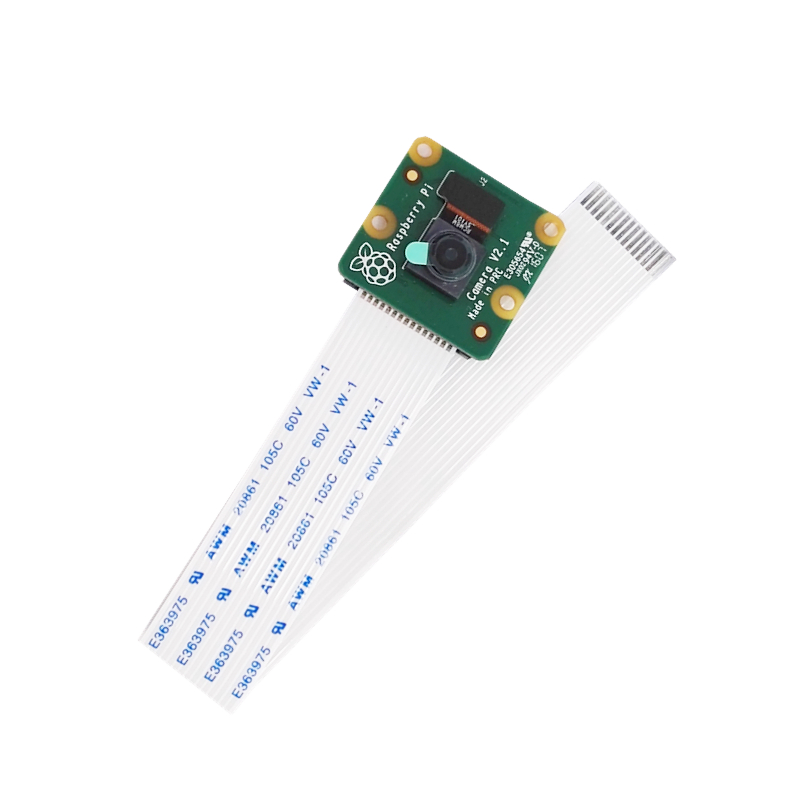
\includegraphics[width = 0.8\textwidth]{Caps/Figs/mat-met/CamRaspberry.jpg}
   \label{fig:sensor-camRaspberry}
    \fonte{Site\protect\footnotemark}
\end{figure}
\footnotetext{Disponível em: \url{https://uploads.filipeflop.com/2017/07/New-Raspberry-Pi-Camera-V2-Video-Module-8MP.jpg}. Acesso em: 8 set. 2020.}

Visão computacional é definida como sendo o conjunto de técnicas computacionais que estimam ou explicitam as propriedades geométricas e dinâmicas do mundo tridimensional a partir de imagens. Trata-se da obtenção automática de informação a respeito do ambiente disponibilizando-a ao sistema de controle, que decidirá qual o comportamento adotar. Utiliza-se de câmeras e plataformas onde essas imagens possam ser processadas, sendo considerado o tipo de informação relevante, a metodologia para extrair a informação e quais as representações empregadas para a atuação do robô.

%================================================================================
\section{Método de Visão Computacional YOLO (\textit{You Only Look Once})}
\label{sec:matmetYOLO}

Sabe-se que o YOLO é um algoritmo baseado em regressão. Isto é, ele não seleciona regiões de interesse da imagem, e sim, prevê classes e caixas delimitadoras para a imagem inteira em uma só execução do algoritmo. Esta implementação é comumente usada para detecção de objetos em tempo real, pois, em geral, eles trocam um pouco de precisão por grandes melhorias na velocidade~\cite{swiezewski2020}.

O funcionamento básico do YOLO é visto na Figura~\ref{fig:yolo-funcionamento} e dado por:
\begin{enumerate}
    \item O algoritmo divide a imagem em um \textit{grid} de S x S células, que geralmente é uma grade 13x13. Porém, nas últimas implementações tem-se usado o tamanho 19x19. Cada uma dessas células é responsável por fazer a predição de 5 caixas delimitadoras (\textit{bounding boxes}), para caso haja mais de um objeto naquela célula (uma caixa delimitadora descreve o retângulo que cobre o objeto).
    \item Retorna uma pontuação de confiança, isto é, o quanto de certeza o algoritmo tem que aquela caixa delimitadora contém um objeto. Essa pontuação não diz respeito de que tipo de objeto tem ali, apenas diz a respeito do formato da caixa em si. Quanto maior a confiança, mais grossa é a linha desenhada.
    \item Para cada caixa a célula também faz a previsão de uma classe, fornecendo um valor de probabilidade para cada uma das classes possíveis que foram treinadas. Esta previsão é feita na CNN.
    \item O valor de confiança para a caixa delimitadora e a predição da classe são combinados em uma pontuação final.
\end{enumerate}

\begin{figure}[!hbtp]
  \centering
   \caption{Modelo de detecção do YOLO.}
    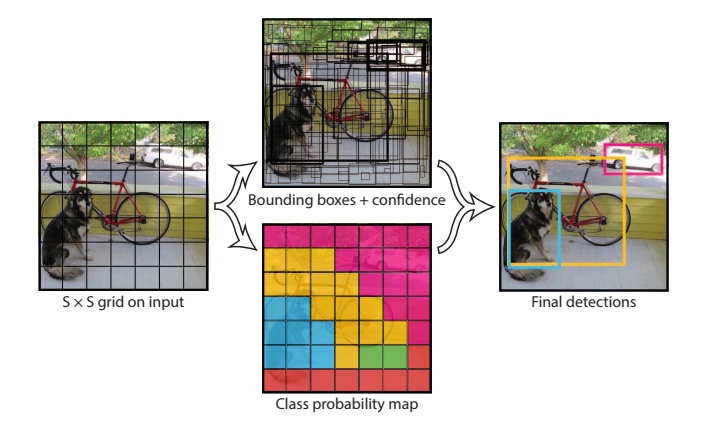
\includegraphics[width = 0.8\textwidth]{Caps/Figs/mat-met/YOLO-funcionamento.png}
   \label{fig:yolo-funcionamento}
    \fonte{\cite{Redmon_2016_CVPR}}
\end{figure}

É importante ressaltar que com uma grade 19x19 há 361 células, e para cada uma dessas células são detectados 5 caixas delimitadoras, o que resulta em 1805 no total. A maioria dessas caixas terá um valor de confiança extremamente baixo. Por isso, geralmente são consideradas apenas as caixas cuja pontuação final seja 30 por cento ou mais (\textit{threshold}).

\subsection{Caixas Delimitadoras (\textit{Bounding Boxes})}
\label{subsec:boundingboxes}

\citeauthor{swiezewski2020} (\citeyear{swiezewski2020}) descreve cada caixa delimitadora em 4 variáveis, estas são:
\begin{itemize}
    \item Centro da caixa delimitadora ($b_x$, $b_y$);
    \item Largura ($b_w$);
    \item Altura ($b_h$);
    \item Valor $c$, que é a classe correspondente ao objeto (pessoa, carro, etc).
\end{itemize}

Deve-se também considerar a probabilidade de existir um objeto na caixa delimitadora, que é representado como valor $p_c$.

\begin{figure}[!hbtp]
  \centering
   \caption{Caixas delimitadoras (\textit{bounding boxes}).}
    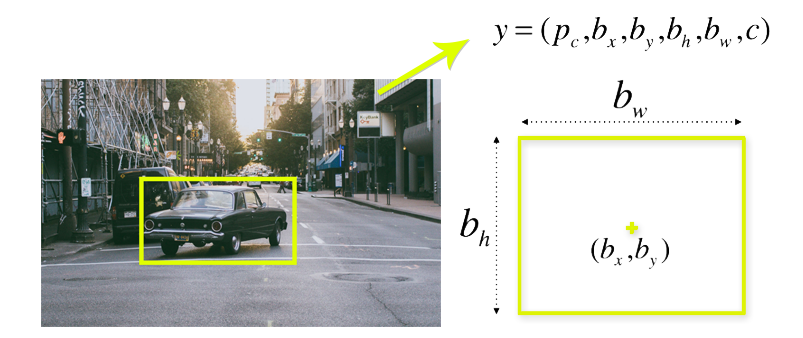
\includegraphics[width = 0.8\textwidth]{Caps/Figs/mat-met/bbox-1.png}
   \label{fig:bbox1}
    \fonte{\cite{swiezewski2020}}
\end{figure}

\begin{figure}[!hbtp]
  \centering
   \caption{Estrutura de definição das \textit{bounding boxes}.}
    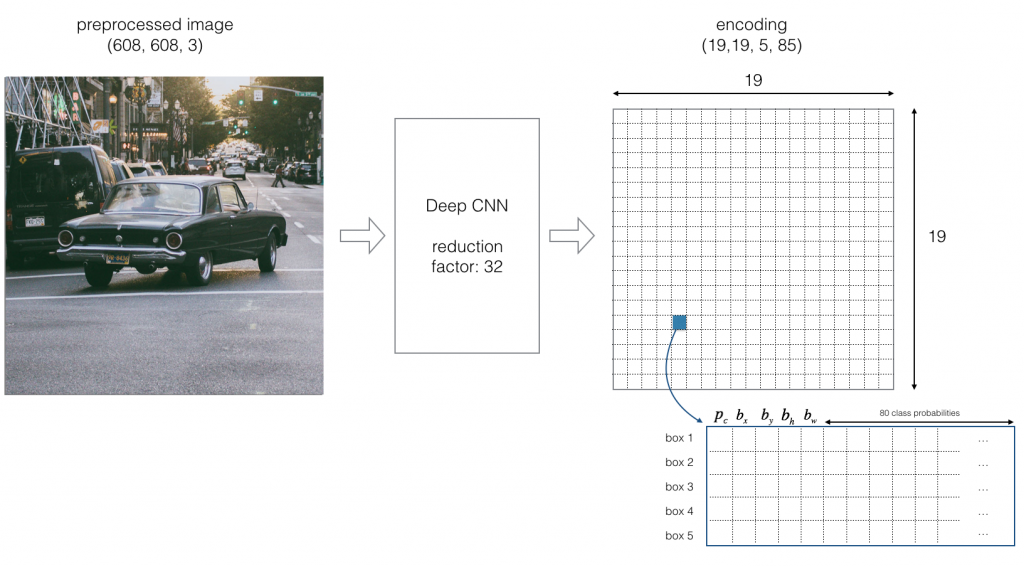
\includegraphics[width = 0.8\textwidth]{Caps/Figs/mat-met/bbox-2.png}
   \label{fig:bbox2}
    \fonte{\cite{swiezewski2020}}
\end{figure}

Na Figura~\ref{fig:bbox2}, observa-se o formato da estrutura (\textit{encoding}) da grade 19x19. Em cada célula vemos as cinco \textit{bounding boxes}, e para cada uma delas a probabilidade de existir um objeto ($p_c$), as variáveis descritivas ($b_x$, $b_y$, $b_w$, $b_h$) e oitenta probabilidades de classe. Originalmente o YOLO foi treinado com uma base de dados chamada COCO~\cite{lin2014microsoft}, e nela existem oitenta objetos diferentes.

\subsection{Supressão Não-Máxima (\textit{Non-Max Supression})}
\label{subsec:nonmax-supression}

Um conceito importante sobre YOLO é a supressão não-máxima. Está técnica é implementada utilizando a biblioteca OpenCV (Seção~\ref{sec:opencv}). A maioria das células não vai conter um objeto, portanto, é necessário obter o valor $p_c$, que servirá para remover caixas com baixa probabilidade de conter um objeto e também caixas que possuem uma área compartilhada.

\begin{figure}[!hbtp]
  \centering
   \caption{Supressão não-máxima (\textit{Non-Max Supression}).}
    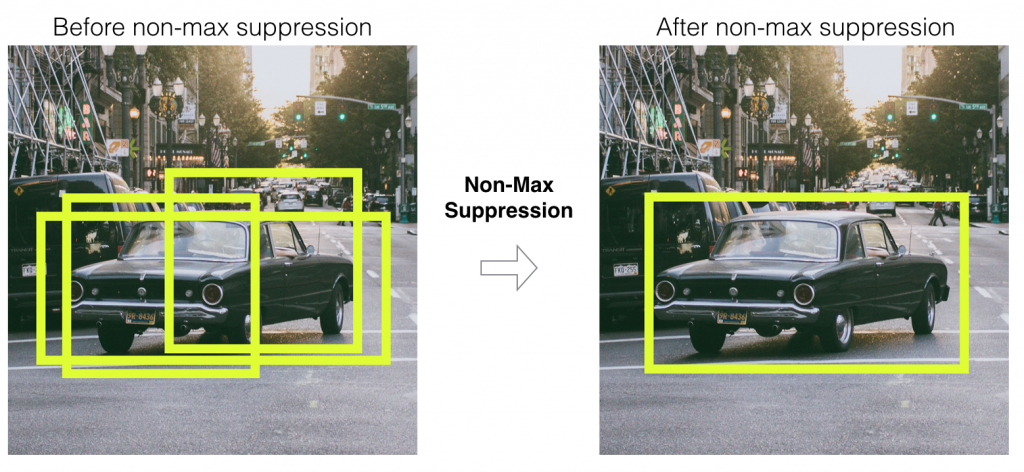
\includegraphics[width = 0.8\textwidth]{Caps/Figs/mat-met/nonmax-1-1024x472.png}
   \label{fig:nonmax-supression}
    \fonte{\cite{swiezewski2020}}
\end{figure}

\subsection{Âncoras (\textit{Anchor Boxes})}
\label{subsec:anchorboxes}

As âncoras (\textit{anchor boxes}), são retângulos de proporções pré-definidas usados para ter maior correspondência entre as caixas delimitadoras previstas e esperadas. Isto é, este algoritmo tem um conjunto de caixas delimitadoras para objetos específicos, que possuem tamanhos iniciais próximos aos tamanhos do objetos e serão redimensionados para o tamanho do objeto usando algumas saídas da rede neural. A CNN não deve prever o tamanho final do objeto, mas ajustar o tamanho da âncora mais próxima ao tamanho do objeto.

O uso de âncoras torna o processo de aprendizagem mais fácil e permite a detecção em várias escalas especificando âncoras de tamanho variados.